\documentclass[12pt]{article}
\usepackage{amsmath,amsfonts,bbm,xfrac}
\usepackage{fancyhdr,enumitem,xcolor,placeins,subcaption,hyperref}
\usepackage{graphicx} % Allows including images
\usepackage[left=2.5cm, right=2.5cm, top =3cm, bottom = 3cm]{geometry}
\hypersetup{
    colorlinks=true,
    linkcolor=blue,
    filecolor=blue,      
    urlcolor=blue,
    }	
\setcounter{MaxMatrixCols}{10}
	
	
	
\pagestyle{plain}
\pagestyle{fancy} 
\rhead{Winter 2023} 
\chead{} 
\lhead{ECON 33530 - Firm Dynamics and Economic Growth} 
\lfoot{} 
\cfoot{} 
\rfoot{\thepage} 
\renewcommand{\headrulewidth}{0.5pt} 
\renewcommand{\footrulewidth}{0pt} 

\title{Firm Dynamics and Economic Growth \\ \large{Problem Set II}}
\author{Jose M. Quintero\thanks{Full replication code can be found at \url{https://github.com/jmquintero925/FD-EG-Ufuk}}}

\begin{document}

\maketitle

The figure is presented here
\begin{figure}[htb]
\centering
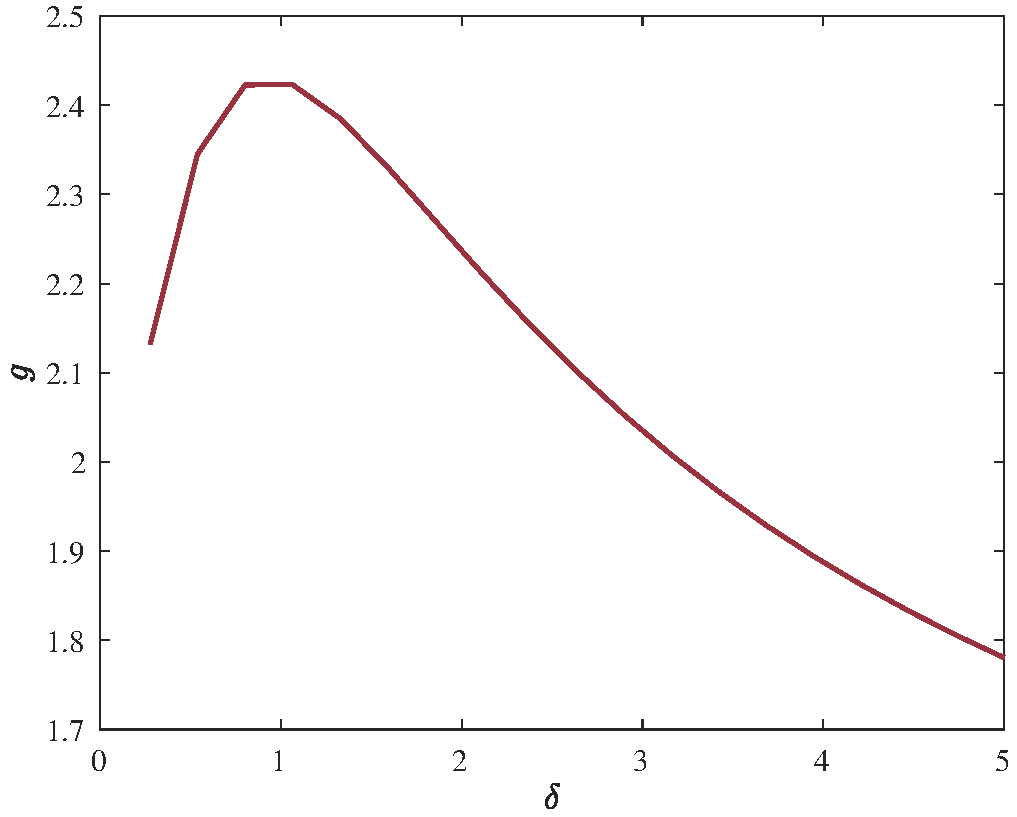
\includegraphics[width=0.6\textwidth]{Figures/figure8.pdf}
\end{figure}
The figure is indeed an inverted U and the value used in the paper $\delta=0.0278$ is in the upward part of the U-shape. The decline in the parameter $\delta$ as suggested by the paper explains why growth and U.S business dynamism has fallen over time. 
\end{document}